% !TEX root = ../foundations.tex

\section{Geometric chains and cochains}\label{S: geometric cochains}

Geometric homology and cohomology are homology/cohomology theories for smooth manifolds defined through submanifolds or, more generally, maps from manifolds with corners.
They agree with singular homology and cohomology, but having different representatives
at the chain/cochain level, they provide geometric approaches to both theory and calculations.
They are thus akin to de Rham theory in the sense that chains and cochains are defined through the smooth structure rather than continuous maps or open sets, but they are defined over the integers and not just the real numbers.

Our definitions of geometric chains and cochains will be a modification of those given by Lipyanskiy in \cite{Lipy14}, though his results will continue to hold with our modified definitions.
As Lipyanskiy primarily focuses on geometric chains and geometric homology, our focus, where the theories diverge, will primarily be on geometric cochains and cohomology, for which Lipyanskiy's account is much less complete despite the cohomological setting having its own subtleties.
We also take the opportunity to fill in some of the details missing from Lipyanskiy's account more generally, especially utilizing the more thorough foundations on manifolds with corners provided by Joyce \cite{Joy12}.

\subsection{Preliminary definitions}

We first identify certain types of ``manifolds over $M$.'' In future sections $M$ will most typically be a manifold without boundary, as that is the case where we obtain agreement between geometric (co)homology and singular (co)homology, but in this section (and anywhere else we do not require transversality of maps to $M$), we allow it to be a manifold with corners anywhere that the extra generality may be useful but so long as it does not create more technical work (such as when utilizing smoothing, as happens below).
In this case, we may interpret ``smooth'' to mean either ``smooth'' or ``weakly smooth'' in the sense of \cite{Joy12}, so long as we are consistent in this interpretation.

\begin{definition}\label{V: maps are co-oriented}
	A \textbf{manifold over $\mathbf{M}$} is a manifold with corners $W$ with a smooth map $r_W \colon W \to M$,
	called the \textbf{reference map}.
	We freely and almost always abuse notation
	by using the domain $W$ to refer to the manifold over $M$, not $r_W$ or some other symbol, letting
	context determine whether we are referring to the entire data or the domain.

	We say a manifold over $M$ is:
	\begin{itemize}
		\item \textbf{compact} if the domain $W$ is compact,
		\item \textbf{proper} if the reference map is proper (if $K \subset M$ is compact then $r_W^{-1}(K)$ is compact),
		\item \textbf{oriented} if $W$ is oriented,
		\item \textbf{co-oriented} if the reference map $r_W$ is co-oriented.
	\end{itemize}
	If $W$ is a manifold over $M$ then so is $\bd W$ using the reference map $r_W \circ i_{\bd W} \colon \bd W \to M$.
	If $W$ is oriented or co-oriented, then $\bd W$ inherits an orientation or co-orientation as in \cref{Con: oriented boundary} or \cref{D: boundary co-orientation}.
	By [Lemma 2.8]{Joy12}, $i_{\bd W}$ is proper, so, as the composition of proper maps is proper, if $W$ is a proper manifold over $M$ then so is $\bd W$.

	If $W$ is oriented or co-oriented we write $-W$ to refer to the manifold over $M$ with the opposite orientation or co-orientation; it should always be clear from context which structure we are replacing with its opposite.
\end{definition}

%The most important case of manifolds over $M$ are submanifolds.
%At times we also employ the notation $W \to M$, to address general maps but keep the emphasis on the case of embeddings.

Geometric chains and cochains will be equivalence classes of manifolds over $M$ under an equivalence relation we define using the following concepts, which are taken from or modify
the definitions of \cite{Lipy14}.

\begin{definition}\label{D: equiv triv and small}
	Let $V, W$ be manifolds over $M$ with reference maps $r_V$ and $r_W$.
	\begin{itemize}
		\item If $V$ and $W$ are oriented, we say they are \textbf{(oriented) isomorphic} if there is an orientation-preserving preserving diffeomorphism $\phi \colon W \to V$ such that $r_V \circ \phi = r_W$.
		If $V$ and $W$ are co-oriented, we say they are \textbf{(co-oriented) isomorphic} if there is a diffeomorphism $\phi \colon W \to V$ such that $r_V \circ \phi = r_W$ and the composition of the
		co-orientation induced by $\phi$
		with the co-orientation of $r_V$ agrees with the co-orientation of $r_W$.

		\item If $W$ is oriented then $W$ is \textbf{(oriented) trivial} if there is an orientation-reversing
		diffeomorphism $\rho \colon W \to W$ such that $r_W \circ \rho = r_W$.
		If $W$ is co-oriented then it is \textbf{(co-oriented) trivial} if there is a diffeomorphism $\rho \colon W \to W$ such that $r_W \circ \rho = r_W$ and
		the composite of the co-orientation induced by $\rho$ with the co-orientation of $r_W$ is the opposite of the co-orientation of $r_W$.
		We call such a map $\rho$ \textbf{co-orientation reversing}.

		\item $W$ has \textbf{small rank} if the differential $D r_W$ is less than full rank everywhere.
		\item If $W$ is (co-)oriented, then it is \textbf{((co-)oriented) degenerate} if it has small rank and ${\bd W}$ is the disjoint union of a trivial (co-)oriented
		manifold over $M$ and one with small rank.
	\end{itemize}
\end{definition}

Note that isomorphism (oriented or co-oriented) is an equivalence relation and that is preserves triviality and degeneracy (oriented or co-oriented, respectively).

Rather than small rank, Lipyanskiy uses the condition of \textbf{small image}.
In our notation, a map $r_W \colon W \to M$ has small image if there is another map $r_T \colon T \to M$ such that $r_T(T)\supset r_W(W)$ but $\dim(T)<\dim(W)$.
However, the small rank condition turns out to be more manageable for our purposes while still providing geometric homology and cohomology theories that are equivalent to singular homology and cohomology.
Roughly speaking, the geometric chains and cochains of a manifold $M$ will consist of isomorphism classes of oriented or proper co-oriented manifolds with corners over $M$ modulo the trivial and degenerate chains and cochains.
The most obvious use of the notion of triviality will be to ensure that $\bd^2 = 0$ so that we have a chain complex.
The degeneracy comes into play in ensuring that geometric homology and cohomology satisfy the dimension axiom; see \cref{E: dimension} and \cref{R: degen1}.

\begin{example}
	Let $S^1$ be the unit circle in the plane with the standard counterclockwise orientation.
	Let $\pi: S^1 \to \R$ be the projection of the circle onto the $x$-axis.
	This map is trivial.
	Indeed, if $\rho$ is the reflection of the circle across the $x$-axis, then $\rho$ is orientation-reversing and $\pi \rho = \pi$.

	Alternatively, let $\pi \colon S^1 \to \R$ be co-oriented by $(e_\theta,e_x)$, where $e_x$ is the standard positively-directed unit vector in $\R$ and $e_\theta$ is the counterclockwise tangent vector in $S^1$.
	This map is trivial as a co-oriented map, again via the reflection $\rho$ across the $x$-axis.
	Indeed, we still have $\pi \rho = \pi$, and the co-orientation induced by $\rho$ is $(e_\theta,-e_\theta)$ so that the composite co-orientation of $\pi\rho$ is $-(e_\theta,e_x)$.
\end{example}

\begin{example}
	If $r_V \colon V \to M$ is any oriented or co-oriented map and $-r_V \colon V \to M$ is the same map with the opposite orientation or co-orientation, then $r_V \sqcup -r_V$ is trivial, taking $\rho$ to be the map that switches the two copies of $V$.
	To be technically accurate, we should not think of a single instance of $V$ as being the domain for both maps in order for $r_V \sqcup -r_V$ to have a well-defined domain that is a submanifold of some $\R^N$.
	However, recall that we are always free to replace $r_V \colon V \to M$ with an isomorphic map whose domain is another, diffeomorphic, ``copy'' of $V$ in $\R^N$.
\end{example}

\begin{example}
	Any co-oriented map of the interval to a point has small rank, but its boundary does not have small rank; it is nonetheless (co-oriented) degenerate because its boundary is trivial.
\end{example}

\begin{example}\label{E: projected triangle}
	Let $V$ be the $2$-simplex in $\R^2$ with vertices at $(1,0)$, $(-1,0)$, and $(0,1)$, and let $\pi \colon V \to \R$ be the projection to the $x$-axis.
	This map has small rank, but the boundary does not have small rank and is not trivial.
\end{example}

\begin{example}
	Let $V = W = M = \R^1$.
	Let $r_W \colon W \to M$ be the identity map of $\R^1$ with the canonical co-orientation, which we can write $(e_1,e_1)$, letting $e_1$ be a positively-oriented tangent vector to $\R^1$.
	Let $r_V \colon V \to M$ be given by $g(t) = -t$ with co-orientation $(-e_1,e_1)$.
	Let $\phi \colon W \to V$ be given by $\phi(t) = -t$.
	Then the canonical co-orientation of $\phi$ is $(e_1,-e_1)$.
	Then $r_V\phi = r_W$ as co-oriented maps, so $\phi$ provides a co-oriented equivalence between $r_W$ and $r_V$ even though they are very different maps.
\end{example}

\subsection{Geometric homology and cohomology}

\begin{definition}
	Denote by $PC^\Gamma_*(M)$ the set of oriented isomorphism classes of compact oriented manifolds over $M$, $r_W \colon W \to M$,
	graded by dimension $\dim(W)$.
	Denote by $PC_\Gamma^*(M)$ the set of co-oriented isomorphism classes of proper co-oriented manifolds over $M$, $r_W \colon W \to M$,
	graded by \textbf{codimension} $\dim(M) - \dim(W)$.
	We declare the empty manifold of each dimension to be orientable and the empty maps from the empty manifolds to $M$ to be co-orientable.

	As per \cref{V: maps are co-oriented}, we will often write $W \in PC^\Gamma_*(M)$ or $W \in PC_\Gamma^*(M)$, letting the reference map be tacit.
	In these respective cases we write $-W$ for $W$ with the opposite orientation or co-orientation.

	We will sometimes refer to elements of $PC^\Gamma_*(M)$ or $PC_\Gamma^*(M)$ as \textbf{prechains} and \textbf{precochains} respectively, and we tend to abuse notation by letting a given map $r_W \colon W \to M$ stand for its isomorphism class.
\end{definition}

For the following definition only we will write isomorphism classes as $[W]$.
In what follows we will abuse notation and refer to such an equivalence class only by a chosen representative.

\begin{definition}
	If $V,W$ are compact oriented manifolds over $M$ (respectively proper co-oriented manifolds over $M$), then define $[V] \sqcup [W] = [V' \sqcup W']$, where on the right $\sqcup$ denotes disjoint union and $V'$ and $W'$ are compact oriented manifolds over $M$ (respectively proper co-oriented manifolds over $M$) such that $V'$ and $W'$ are disjoint in $\R^\infty$ (cf.
	\cref{D: MWC}).
\end{definition}

The last clause in the definition is due to our requirement that all manifolds with corners be subsets of $\R^\infty$.
As given, the definition allows constructions like $[W]\sqcup[W]$ to be well defined.
We observe that this definition is well defined in general, since if $V''$ and $W''$ are two other manifolds over $M$ isomorphic to $V$ and $W$ (in the appropriate sense), then we can compose the diffeomorphisms $V'\xleftarrow{\phi'}V \xr{\phi''} V''$ and $W'\xleftarrow{\psi'}W \xr{\psi''} W''$ to obtain an isomorphism $\phi''(\phi')^{-1} \sqcup \psi''(\psi')^{-1} \colon V' \sqcup W' \to V'' \sqcup W''$.

With $\sqcup$, $PC^\Gamma_*(M)$ and $PC_\Gamma^*(M)$ become commutative monoids in each degree with the empty maps $r_\emptyset \colon \emptyset \to M$ as the identities.

We now return to denoting isomorphism classes by their representatives, noting again that triviality and small rank are properties of the isomorphism classes.

\begin{definition}
	Let $Q_*(M) \subset PC_*(M)$ denote the set of (isomorphism classes of) compact oriented manifolds over $M$ of the form $V \sqcup W$ with $V$ trivial and $W$ degenerate.
	Let $Q^*(M) \subset PC^*(M)$ denote the set of (isomorphism classes of) proper co-oriented manifolds over $M$ of the form $V \sqcup W$ with $V$ trivial and $W$ degenerate.
	In either case $V$ or $W$ may be empty.

	We will sometimes write $W \in Q(M)$ to mean $W \in Q_*(M)$ or $W \in Q^*(M)$ for arguments that are analogous in the two cases.
	When we do so, we assume a consistent choice of $Q_*(M)$ or $Q^*(M)$ throughout the discussion; see for instance \cref{L: bd defined} and its proof.
\end{definition}

The following useful basic properties are proven in \cite{Lipy14}; for completeness we provide versions of the arguments here, occasionally augmenting those of \cite{Lipy14}.
In each case, ``isomorphic,'' ``trivial,'' or ``degenerate'' should be read consistently to refer to the compact oriented case or the proper co-oriented case.
Lipyanskiy's proofs assume small image rather than small rank, butthe proofs are equivalent.

\begin{lemma}[Lipyanskiy Lemma 10]\label{L: Lip L10}
	If $V$ is trivial and $V \sqcup W$ is trivial, then $W$ is trivial.
\end{lemma}

\begin{proof}
	We can write $W$ as the disjoint union of a (possibly infinite) number of isomorphism classes of connected components and then group the isomorphism classes together up to (co-)orientation as $W = W_1 \sqcup W_2 \sqcup \cdots$ so that all connected components of each $W_i$ are isomorphic (ignoring (co-)orientations) for each $i$ and so that no connected component of $W_i$ is isomorphic to a connected component of $W_j$ for $i\neq j$.
	As either $W$ is compact or $r_W$ is proper, each $W_i$ is the union of a finite number of connected components.
	Any automorphism of $W$ preserves the decomposition into $W_i$ and so $W$ is trivial if and only if for all $i$ either $W_i$ has zero components when counting with (co-)orientation or each component of $W_i$ has a (co-)orientation reversing automorphism.

	Similarly, since $V$ is trivial, $V$ can be decomposed into unions of isomorphism classes, up to (co-)orientation, of connected components with $0$ components when counting with sign or with all components having (co-)orientation reversing automorphisms.
	In particular, forming $V \sqcup W$ adds to $W$ zero components when counting with sign or components with (co-)orientation reversing automorphisms, so if $V \sqcup W$ is trivial, $W$ must have already been trivial.
\end{proof}

\begin{lemma}[Lipyanskiy Lemma 11]\label{L: bd defined}
	If $W$ is in $Q(M)$, then $\bd W \in Q(M)$.
\end{lemma}

\begin{proof}
	We first check that if $W$ is trivial then so is its boundary $r_{\bd W} = r_Wi_{\bd W} \colon \bd W \to M$.
	If $\rho \colon W \to W$ is (co-)orientation reversing, then we can consider $\rho_\bd$ as defined in \cref{R: bd diff}.
	As $r_W\rho = r_W$ we also have $r_Wi_{\bd W} = r_W\rho i_{\bd W} = r_W i_{\bd W} \rho_\bd$.
	Thus we only need see that $\rho_\bd$ is orientation reversing.
	It is sufficient to consider what happens at points on the interior of $\bd W$ so working locally we may identify such points of $\bd W$ with points of $W$ itself and similarly identify $\rho_\bd$ with $\rho$.
	In the oriented case, the orientation of $W$ determines orientations of $T_xW$ and $T_{\rho(x)}W$, and by assumption $D\rho: T_xW \to T_{\rho(x)}W$ takes the orientation of $T_xW$ to the opposite of the orientation of $T_{\rho(x)}W$.
	But also $D\rho$ must preserve inward/outward pointing vectors.
	Thus $D\rho$ must restrict to a map $T_x (\bd W) \to T_{\rho(x)}(\bd W)$ that also reverses the orientation.
	The co-oriented situation is analogous using local orientation pairs $\left(\beta_{W,x}, \beta_{M,r_W(x)}\right)$ and $\left(\beta_{W,\rho(x)}, \beta_{M,r_W\rho(x)}\right)$ and taking $\beta_{M,r_W\rho(x)} = \beta_{M,r_W(x)}$ as $\rho$ is a diffeomorphism over $M$.

	Now suppose $W$ degenerate.
	By definition $\bd W = A \sqcup B$ with $A$ trivial and $B$ of small rank.
	Then $\bd^2 W = \bd A \sqcup \bd B$.
	As noted, $\bd A$ is trivial, and $\bd^2 W$ is trivial for all $W$ by \cref{L: boundary2}.
	It follows from \cref{L: Lip L10} that $\bd B$ is trivial, and so $B$ is degenerate.
	Thus $\bd W$ is degenerate.
\end{proof}

\begin{lemma}[Lipyanskiy Lemma 12]\label{L: Lipy12}
	If $V$ and $V \sqcup W$ are in $Q(M)$, then $W \in Q(M)$.
\end{lemma}

\begin{proof}
	As in the proof of \cref{L: Lip L10}, decompose $W$ as $W = W_1 \sqcup W_2 \sqcup \cdots$ and $V$ as $V = V_1 \sqcup V_2 \sqcup \cdots$.
	As $V$ and $V \sqcup W$ are in $Q(M)$, each $V_i$ has small rank or, also as in the proof of \cref{L: Lip L10}, $V_i$ is trivial, and similarly for $V \sqcup W$, from which it follows again by counting with signs in the trivial components that each $W_i$ is either trivial or has small rank.
	By grouping terms of the decomposition we can write $W = A \sqcup B$ with $A$ trivial and $B$ of small rank.

	We then have $\bd V$ and $\bd (V \sqcup W) = \bd V \sqcup \bd A \sqcup \bd B$ in $Q(M)$ by \cref{L: bd defined}, and also $\bd A$ is trivial as the boundary of a trivial manifold over $M$ by \cref{L: bd defined}.
	Now by the same argument as in the previous paragraph, replacing $V$ with $\bd V \sqcup \bd A$ and $W$ with $\bd B$, we have that $\bd B$ can be decomposed into the disjoint union of a trivial manifold over $M$ and one with small rank.
	But this shows $B$ is degenerate, so $W \in Q(M)$.
\end{proof}

\begin{lemma}[Lipyanskiy Lemma 13]\label{L: cancel Q}
	The relation given by $V\sim W$ if $V \sqcup -W$ is in $Q_*(M)$ (respectively $Q^*(M)$) is an equivalence relation on $PC^\Gamma_*(M)$ (respectively $PC_\Gamma^*(M)$).
\end{lemma}

\begin{proof}
	Reflexivity: For any $W$, we have $W \sqcup -W$ trivial via the map that interchanges the two copies of $W$.

	Symmetry: If $V \sqcup -W$ is the union of trivial and degenerate manifolds over $M$ then certainly so is $W \sqcup -V = -(V \sqcup -W)$.

	Transitivity: If $V \sqcup -W$ and $W \sqcup -U$ are in $Q_*(M)$ (or $Q^*(M)$), then so is $V \sqcup -W \sqcup W \sqcup -U \cong V \sqcup -U \sqcup W \sqcup -W$.
	We know $W \sqcup -W$ is trivial, and so $V \sqcup -U$ is in $Q_*(M)$ (or $Q^*(M)$) by \cref{L: Lipy12}.
\end{proof}

These lemmas allow us to follow Lipyanskiy in defining geometric chains and cochains.
We will show that the claims of the following definition hold in \cref{L: co/chains well defined} just below.

\begin{definition}
	The \textbf{geometric chains} of $M$, denoted $C^\Gamma_*(M)$, are the $\sim$ equivalence classes in $PC^\Gamma_*(M)$.
	The \textbf{geometric cochains} of $M$, denoted $C_\Gamma^*(M)$, are the $\sim$ equivalence classes in $PC_\Gamma^*(M)$.
	These are chain complexes under the operation $\sqcup$ and with boundary map $\bd$.

	In either case we denote the equivalence class of $W$ by $\uW$, and $\uW = 0$ in $C^\Gamma_*(M)$ (respectively $C_\Gamma^*(M)$) if and only if $W$ is in $Q_*(M)$ (respectively $Q^*(M)$).

	We define the \textbf{geometric homology} of $M$, written $H_*^\Gamma(M)$, to be $H_*(C^\Gamma_*(M))$, and
	we define the \textbf{geometric cohomology} of $M$, written $H^*_\Gamma(M)$ to be $H^*(C_\Gamma^*(M))$.
\end{definition}

The notation says that if $V$ and $W$ represent equivalence classes $\uV$ and $\uW$, then in $C_*^{\Gamma}(M)$ (or $C^*_\Gamma(M)$), we have $\uV+\uW = \underline{V \sqcup W}$.
In particular every chain or cochain can be represented by a single map $r_W \colon W \to M$ for appropriate $W$.
Similarly, $V \in Q_*(M)$ (or $Q^*(M)$) if and only if $\uV = 0$.

\begin{lemma}\label{L: co/chains well defined}
	The chain complexes $C_\Gamma^*(M)$ and $C_\Gamma^*(M)$ are well defined with $\uW = 0$ in $C^\Gamma_*(M)$ (respectively $C_\Gamma^*(M)$) if and only if $W$ is in $Q_*(M)$ (respectively $Q^*(M)$).
\end{lemma}

\begin{proof}
	This is a consequence of the preceding lemmas.
	For simplicity we work with $Q_*(M)$ and $C^\Gamma_*(M)$, but the identical arguments hold with $Q^*(M)$ and $C_\Gamma^*(M)$.

	Addition is well defined because if $\uV,\uW \in C^\Gamma_*(M)$ with $V$ and $V'$ in the class $\uV$ and $W$ and $W'$ in the class $\uW$, then $\uV+\uW$ is well defined as the class $\underline{V \sqcup W}$ because $(V \sqcup W) \sqcup -(V' \sqcup W') = (V \sqcup -V') \sqcup (W \sqcup -W')$: By assumption $V \sqcup -V' \in Q_*(M)$ is the disjoint union of a trivial manifold over $M$ and a degenerate manifold over $M$, and similarly for $W \sqcup -W'$, so $(V \sqcup -V') \sqcup (W \sqcup -W') \in Q_*(M)$.

	The identity in each degree is represented by $\emptyset$ with the unique empty map to $M$ (with either orientation or co-orientation).
	In fact, every element of $Q_*(M)$ represents $0$ in $C^\Gamma_*(M)$ as elements of $Q_*(M)$ are all equivalent to $\emptyset$.
	Conversely, if $\uW = 0$ then $W \in Q_*(M)$, as if $\uV+\uW = \uV$ then $V \sqcup W \sqcup -V \in Q_*(M)$.
	But $V \sqcup -V \in Q_*(M)$, so by \cref{L: Lipy12}, $W \in Q_*(M)$.
	We also see that the additive inverse of $\uW$ is $\underline{-W}$, as $W \sqcup -W$ is trivial.

	That the boundary map is well defined with $\bd \uW = \udW$ is due to \cref{L: bd defined} and \cite[Lemma 2.8]{Joy12}, which implies that $\bd W$ is proper.
	That $\bd^2 = 0$ in the case of cochains follows from \cref{L: boundary2}, which shows that $\bd^2 W$ is always trivial.
	Similarly, to obtain $\bd^2 = 0$ for chains see \cref{R: bd2 oriented}.
\end{proof}

\begin{comment}
	Thom deeply considered the interplay between manifolds
	and homology \cite{Thom54}, and the cohomology classes we produce for submanifolds are equal to the pullbacks of Thom classes by Thom collapse maps.
	Similar objects were defined by Quillen \cite{Quil71} as an immediate translation of the data which encodes cobordism generalized cohomology theories.
	Thus, we name the QT-objects which represent equivalence classes of geometric cochains, defined below, in honor of Quillen and Thom.
\end{comment}

\begin{comment}
	If $i \colon W \to M$ is an embedding of a submanifold,
	we abuse notation by referring to the cochain as $\tau_W$, suppressing the reference map from the notation.
	Indeed, the image of any $\tau_i$ under our comparison map to cubical cochains will be the same.
\end{comment}

\begin{comment}
	%Geometric reasoning is aided by focussing on the image of the map rather than the map itself.
\end{comment}

\begin{comment}
	Having given our version of geometric chains and cochains, for the remainder of this section we work exclusively with cochains, referring to \cite{Lipy14}for (or leaving as exercises for the interested reader) the analogous properties of geometric chains.

	\begin{lemma}
		Geometric chains and cochains on $M$ form chain complexes --- that is, $d^\Gamma$ and $d_\Gamma$ square to zero.
	\end{lemma}

	This lemma is essentially Lemma~13 of \cite{Lipy14}.
	The key is that while $\bd^2 W$ is not empty,

	BCOMMENT
	, nor is it zero at the level of pre-cochains
	ECOMMENT
	it is trivial.
	That is, it has a $C_2$-action, permuting the local boundary components attached to points in $S^2(W)$.
	Moreover, under our co-orientation conventions, the two vectors appended to the co-orientation of $W$ to obtain one for $\bd^2 W$ over the same point in
	$S^2(W)$ differ by a transposition, so this $C_2$-action is co-orientation reversing.
	This fact about $\bd^2$ not only eventually shows that $d_\Gamma^{\,2} = 0$, but is first needed to show that the boundary of a degenerate map is degenerate; \red{see the proof of \cite[Lemma 11]{Lipy14}}.
\end{comment}

\begin{comment}
	\red{Reflecting on all of these definitions, an illustrative example of a manifold over $M$ defined by a proper map
		is given by embedding the positive $x$-axis within $\R^3 \setminus \{0\}$, \red{together with a choice of orientation of its normal bundle}, which represents a generator of the second cohomology [GBF: I modified this example to make it clearer that we index by codimension, since none of the previous examples really showed that off.]}.
	Another illustrative example is given by a linear embedding of $\R P^2$ into $\R P^4$.
	The domain manifold is not orientable, but the map is co-orientable and represents a nonzero class in $H^2(\R P^4; \Z)$.
	\red{[GBF: How do we know this class is non-zero? Can we prove that?]}
	We also recall that Schubert subvarieties of Grassmannians are not smooth, but do have standard
	smooth resolutions with reference maps to Grassmannians which can used to represent cohomology.
\end{comment}

\begin{comment}
	In Section 6 of \cite{Lipy14}, Lipyanskiy shows that the homology of $C_\Gamma^*(M)$, which we denote by $H_\Gamma^*(M)$,
	agrees with singular cohomology
	through the verification of homotopy and excision axioms.
	We find Mayer-Vietoris better for our applications, and we review both its verification
	and that of homotopy invariance as we need details about such constructions in our work.
\end{comment}

In Section 6 of \cite{Lipy14}, Lipyanskiy shows that the homology theory based on geometric chains satisfies some of the Eilenberg-Steenrod axioms.
This is enough to state in Section 10 of \cite{Lipy14} that geometric homology is isomorphic to singular homology on the fixed manifold $M$, though we provide our own proof below.
Unfortunately, Lipyanskiy does not provided a detailed treatment of geometric cohomology, which is different from geometric homology in several respects, though we will also show that it is isomorphic to singular cohomology.

First, though, we present here some computational examples, mostly without proofs, to aid the reader's intuition.

\begin{example}\label{E: first examples}
	For any manifold, the map of an oriented point to $M$ is a generator of $H_0^\Gamma(M)$.
	Any two points with the same orientation mapping to the same component of $M$ represent the same element of $H_0^\Gamma(M)$ as can be seen by joining them with a smooth path.

	The generators of $H^0_\Gamma(M)$ are the inclusions of the connected components with the tautological co-orientations.

	If $M$ is close and oriented with $\dim(M) = m$ then $H_m^\Gamma(M)$ is generated by the inclusions of connected components.

	Elements of $C_\Gamma^m(M)$ are represented by co-oriented maps of points to $M$.
	If $M$ is compact such a map is a generator of a non-trivial cohomology class.
	If the point maps to a non-compact component of $M$ then it represents $0$ in $H_\Gamma^m(M)$ because any proper path $(-\infty,0] \to M$ with the restriction to $0$ being our cochain representative gives a null-cohomology with appropriate choices of co-orientation.

	In $\R^3-\{0\}$, the inclusion of the positive $x$-axis with either co-orientation is a generator of $H_\Gamma^2(M)$, while the embedding the oriented unit 2-sphere containing the origin is a generator of $H_2^\Gamma(M)$.

	If $M$ is compact and oriented then tautologically $C_*^\Gamma(M) = C_\Gamma^{\dim(M)-*}(M)$.
	This is a strong form of Poincar\'e duality.
\end{example}

\begin{example}[Dimension axiom]\label{E: dimension}
	If $M$ is a point, then every $r_W \colon W \to M$ with $\dim(W)>0$ is degenerate: If $\dim(W)>1$, both $W$ and $\bd W$ must have small rank.
	If $\dim(W) = 1$ then $W$ is a union of closed intervals and circles, so it has small rank, while $\bd W$ is trivial, consisting of pairs of maps $pt \to pt$ with opposite (co-)orientations.
	Thus $C_*^\Gamma(pt) = C^{-*}_\Gamma(pt) = 0$ unless $* = 0$, and so $H_*^\Gamma(pt) = H^{-*}_\Gamma(pt) = 0$ unless $* = 0$.
	When $* = 0$, the identity $pt \to pt$ is a cycle (or cocycle) that does not (co)bound, and as in ordinary bordism theory we have $H_0^\Gamma(pt) \cong H^0_\Gamma(pt) \cong \Z$.
\end{example}

\begin{remark}\label{R: degen1}
	It is in the dimension axiom that we most obviously see the need to include degenerate chains and cochains in $Q(M)$.
	On the other hand, the formulation of degeneracy as given will create some difficult for us in \cref{S: products} when it comes to consider notions of transversality for geometric chains and cochains.
	The reason is that degeneracy causes much of the problematic ambiguity in choosing representatives for chains and cochains.
	For example, consider a connected prechain $V \in PC_*(M)$ with small rank but a boundary that is not in $Q_*(M)$.
	If $V'$ is any other such prechain with small rank and $\bd V = \bd V'$, then $V \sqcup -V' \in Q_*(M)$, so $V$ and $V'$ represent the same chain but could behave wildly differently aside from their boundaries.
	By contrast, we will see in \cref{S: products} that trivial chains are less of an issue (they can generally be ignored) and that non-trivial components without small rank are ``essential'' in a sense we will make precise in \cref{D: essential}; essential components appear in any representative of the same geometric chain or cochain.

	Given the headaches thus caused by the degenerate chains and cochains, it is tempting to ask for a simpler definition of degeneracy.
	One variant that comes to mind would be defining degeneracy so that each individual component must have a boundary consisting of trivial and small rank (co)chains.
	This would seem to be sufficient for the dimension axiom and would eliminate the difficulty described above.
	Unfortunately, with such an alternative definition of degeneracy, it will not generally be true that if $V \in Q(M)$ then fiber products $V \times_M W$ are also in $Q(M)$.
	This is an important property that will arise in the next section and then be needed both to construct cup and cap products and to prove the existence of Mayer-Vietoris sequences.
	See \cref{R: degen2} for further discussion of this point.
\end{remark}

The following algebraic property will be useful below as we consider homological algebra with geometric cochains:

\begin{lemma}
	Each $C_i^\Gamma(M)$ or $C_\Gamma^i(M)$ is torsion-free and hence flat as a $\Z$-module.
\end{lemma}

\begin{proof}
	The second statement follows from the first as $\Z$ is a Dedekind domain.
	The first statement is proven for geometric chains in \cite[Lemma 34]{Lipy14}.
	The proof for geometric cochains, even accounting for our different definition of degeneracy, is the same.
\end{proof}

\subsubsection{Products of manifolds over \texorpdfstring{$M$}{M}}

In this section we define various products of elements of $PC_*^\Gamma(M)$ and $PC^*_\Gamma(M)$, all coming from the external products of fiber products defined above.
These products will ultimately become our cup, cap, intersection, and exterior products, but we introduce them here as products on $PC_*^\Gamma(M)$ and $PC^*_\Gamma(M)$ and derive some further properties as we will need some of this material in the next section to define creasing.
The first time reader can fairly safely skip this section for now and return to it later as needed.

\begin{definition}\label{D: PC products}
	Given a manifold without boundary $M$, the fiber product $(V,W) \to V \times_M W$, with the appropriate corresponding fiber product orientation or co-orientation, determines partially-defined products of the following forms:
	\begin{align*}
		PC^*_\Gamma(M) \times PC^*_\Gamma(M)& \to PC^*_\Gamma(M)\\
		PC^*_\Gamma(M) \times PC_*^\Gamma(M)& \to PC_*^\Gamma(M).
	\end{align*}
	If, furthermore, $M$ is oriented, then there is also a partially-defined product
	$$PC_*^\Gamma(M) \times PC_*^\Gamma(M) \to PC^*_\Gamma(M).$$
	In each case, the product is defined when the reference maps $r_V \colon V \to M$ and $r_W \colon W \to M$ are transverse.
\end{definition}

To define these products, in each case we suppose transverse maps $r_V \colon V \to M$ and $r_W \colon W \to M$ representing elements of
$PC^*_\Gamma(M)$ or $PC_*^\Gamma(M)$ and form the fiber product $V \times_M W \to M$.
Then the first product is well defined by the definition of the fiber product co-orientation, \cref{L: co-orientable pullback}, and that the composition of proper maps is proper.
For the second product, we have the pullback co-orientation $V \times_M W \to W$, and $W$ is compact and oriented by definition.
So $V \times_M W$ is compact by \cref{L: co-orientable pullback} as a proper map to a compact space must have compact domain.
We also recall that given a smooth map of manifolds with oriented codomain, an orientation of the domain determines a co-orientation of the map and vice versa; see the discussion following \cref{D: co-orientations}.
So $V \times_M W$ is compact, and if we give it the orientation we obtain from the pullback co-orientation of $V \times_M W \to W$, we obtain an element of $PC_*^\Gamma(M)$.
For the third map, we use the convention of Joyce recalled in \cref{S: orientations} to oriented a fiber product of oriented manifolds with corners and observe that $V \times_M W$ is compact as a closed subset of the compact $V \times W$.
Thus we obtain an element $PC_*^\Gamma(M)$.
In this last case, we really need $M$ to be oriented in general, as we have observed in \cref{R: what products exist} that if $M$ is not orientable the fiber product of orientable manifolds over $M$ may be non-orientable.

In the cases where $r_V$ and $r_W$ are transverse embeddings, these products are represented by just taking intersections, with the orientations or co-orientations given explicitly in \cref{P: normal pullback,P: cap of immersions,P: orient intersection}.
If $r_V$ and $r_W$ are immersions, these descriptions hold locally.

The next Lemma will be critical in \cref{S: products} toward showing that these products extend to well-defined, though only partially-defined, products of geometric chains and cochains.
It will also be needed much sooner to show that the creasing construction is well defined.
This construction is used, in turn, to demonstrate the existence of Mayer-Vietoris sequences.

\begin{lemma}\label{L: pullback with Q}
	For any of the products above, if either $V$ or $W$ is in $Q(M)$, then $V \times_M W \in Q(M)$.
	In fact, if $V$ or $W$ is trivial then $V \times_M W$ is trivial, and if $V$ or $W$ has small rank then $V \times_M W$ has small rank.
\end{lemma}

\begin{proof}
	We provide the proof if $V \in Q(M)$; the other case is similar.
	By assumption $V$ is the disjoint union of trivial and degenerate chains or cochains, so it suffices to consider independently the possibilities that $V$ is trivial or degenerate.

	If $\rho$ is a (co-)orientation reversing diffeomorphism of $V$ over $M$, then $\rho \times_M \id_W$ is a (co-)orientation reversing diffeomorphism of $V \times_M W$, by Joyce's construction in the oriented case and by \cref{R: co-or restriction or switch} in the co-oriented case.

	Next assume that $V$ is degenerate, so in particular it has small rank.
	Recall that the tangent bundle of a fiber product is the fiber product of the tangent bundles \cite[Theorem 5.47]{Wed16}, and so the derivative is the fiber product of derivatives.
	Note that the fiber product of two linear maps, one with a non-trivial kernel, must also have a non-trivial kernel: If $A,B$ are linear maps with a common codomain and $v \in \ker(A)$, then $(v,0)$ is in the kernel of the fiber product of $A$ and $B$.
	So if the differential of $r_W$ has non-trivial kernel everywhere so will the derivative of any fiber product with $r_W$.
	Thus $V \times_M W$ has small rank.

	Now we recall that $\bd(V \times_M W)$ is, up to (co-)orientations, the union of $(\bd V) \times_M W$ and $V \times_M (\bd W)$.
	We have just shown that $V \times_M (\bd W)$ must have small rank.
	As $V$ is degenerate, $\bd V$ is a disjoint of trivial and small rank manifolds over $M$, and so by the preceding arguments $(\bd V) \times_M W$ will be a union of trivial and small rank manifolds over $M$.
	Altogether, $V \times_M W$ is degenerate.
\end{proof}

\begin{remark}\label{R: degen2}
	As noted in \cref{R: degen1}, it is this lemma that fails if we attempt to simplify the definition of degeneracy by requiring each connected component of a degenerate prechain or precochain to have small rank and boundary that is a union of trivial and small rank pre(co)chains.
	In fact, it is possible to construct a $V$ and $W$ such that $V$ is a non-trivial prechain that is degenerate in this stronger sense but such that $V \times_M W$ has multiple components that are each non-trivial and of small rank but such that the boundary of each component is non-trivial and not of small rank.
	So $V \times_M W$ would not be in a version of $Q(M)$ defined using this stronger, but simpler, notion of degeneracy.
	Of course it is in $Q(M)$ with our actual definitions by the preceding lemma.
\end{remark}

We have a similar result for the exterior products studied in \cref{S: exterior products}, which are always fully defined:

\begin{lemma}\label{L: exterior Q}
	Suppose $f \colon V \to M$ and $g \colon W \to N$ are respectively in $PC_*(M)$ and $PC_*(N)$ or that they are respectively in $PC^*(M)$ and $PC^*(N)$.
	Suppose $V \in Q(M)$ or $W \in Q(N)$.
	Then $f \times g \colon V \times W \to M \times N$ is in $Q(M \times N)$.
\end{lemma}

\begin{proof}
	We provide the proof if both maps are in $PC^*$ and $V \in Q^*(M)$; the other cases are similar.
	By assumption $V$ is the disjoint union of trivial and degenerate chains or cochains, so it suffices to consider independently the possibilities that $V$ is trivial or degenerate.

	If $\rho$ is a (co-)orientation reversing diffeomorphism of $V$ over $M$, then $\rho \times \id_W$ is a (co-)orientation reversing diffeomorphism of $V \times_M W$.
	So if $V$ is trivial so is $V \times W$.

	Next assume that $V$ is degenerate, so in particular it has small rank.
	The derivative of $f \times g$ is matrix with $Df$ and $Dg$ on the block diagonals, so $f \times g$ has small rank.
	Now we recall that $\bd(V \times W)$ is, up to co-orientations, the union of $(\bd V) \times_M W$ and $V \times_M (\bd W)$.
	We have just shown that $V \times_M (\bd W)$ must have small rank.
	As $V$ is degenerate, $\bd V$ is a disjoint of trivial and small rank manifolds over $M$, and so by the preceding arguments $(\bd V) \times_M W$ will be a union of trivial and small rank manifolds over $M$.
	Altogether, $V \times_M W$ is degenerate.
\end{proof}

\begin{comment}
	The next theorem, which is yet another Leibniz formula, in this case for the pullback of a co-oriented manifold over $M$ by an oriented manifolds over $M$, will be used in Section \ref{S: intersection map} to demonstrate that our intersection map $\mc I$, relating geometric cochains to cubical cochains of a cubulation, is a chain map.
	This map is a critical component in relating geometric cohomology to other cohomology theories and is also central to the main result about cup products in \cite{FMS-flows}.

	\begin{theorem}\label{T: Leibniz cap}
		Let $M$ be a manifold without boundary.
		Suppose $V \in PC^*_\Gamma(M)$ and $W \in PC_*^\Gamma(M)$ with transverse reference maps.
		Consider $V \times_M W$ as representing an element of $PC_*^\Gamma(M)$ as constructed in Definition \ref{D: PC products}.
		Then in $PC_*^\Gamma(M)$, $$\bd(V \times_M W) = \left[(-1)^{\dim(V \times_M W)} (\bd V) \times_M W\right] \bigsqcup V \times_M \bd W.$$
	\end{theorem}
	\begin{proof}
		By Definition \ref{D: PC products} the terms $\bd(V \times_M W)$, $(\bd V) \times_M W$, and $V \times_M \bd W$ are each oriented by considering, as appropriate, the pullback of the co-oriented map $V \to M$ or $\bd V \to M$ to a co-oriented map to $W$ or $\bd W$ and then using the orientation of $W$ or $\bd W$ to determine an orientation of the pullback.
		So we compute and compare these orientations by first considering the pullback co-orientations as defined in Definition \ref{D: pullback coorient}.
		We proceed by analogy to the proof of the Leibniz rule for the pullback of co-oriented maps in Theorem \ref{leibniz}, utilizing the computations already performed there.

		Recall, in brief, from \ref{D: pullback coorient} that to co-oriented the pullback $P = V \times_M W \to W$ we first construct a composition $V\xhookrightarrow{e} M \times \R^N \to M$ and find a Quillen orientation for the normal bundle $\nu V$ of $e(V) \subset M \times \R^N$ as determined by the co-orientation of $V \to M$.
		Then we pull back via $W \times \R^N \to M \times \R^N$ to obtain a normal bundle, also labeled $\nu V$, of $P \subset W \times \R^N$.
		Then we co-orient $P \to W$ locally by $(\beta_P,\beta_W)$ so that $\beta_P \wedge \beta_{\nu V} = \beta_W \wedge \beta_E$, where $\beta_E$ represents the standard orientation of $\R^N$.
		In the case at hand, we can assume $\beta_W$ to represent the global orientation of $W$, and then $\beta_P$ becomes a global orientation for $P$.
		This is the orientation given to $V \times_M W$ in Definition \ref{D: PC products}.

		Let $\nu\bd P$ denote an outward pointing normal vector in the tangent bundle to $P$ at a boundary point of $P$, and let $\beta_{\nu\bd P}$ denote the corresponding orientation.
		Then, by definition, $\bd P$ is oriented at that point by $\beta_{\bd P}$ so that $\beta_{\nu\bd P} \wedge \beta_{\bd P} = \beta_P$.
		In other words, with $\beta_P$, $\beta_W$, $\beta_{\nu V}$, and $\beta_E$ given, $\bd P$ is oriented by $\beta_{\bd P}$ such that $\beta_{\nu\bd P} \wedge \beta_{\bd P} \wedge \beta_{\nu V} = \beta_W \wedge \beta_E$.

		Now, recall that $\bd(V \times_M W) = (\bd V) \times_M W \bigsqcup V \times_M \bd W$ as spaces and consider a point in $(\bd V) \times_M W$.
		By Theorem \ref{leibniz}, at such a point the pullback co-orientation of $(\bd V) \times_M W \to W$ agrees with boundary co-orientation of the pullback $P = V \times_M W \to W$, as described again in the preceding paragraph.
		So continuing to let $(\beta_P,\beta_W)$ denote the pullback co-orientation of $P \to W$ and recalling that the boundary co-orientation utilizes the \textit{inward} normal, the boundary co-orientation of $(\bd V) \times_M W \to W$ is the composite $(\beta_{\bd P}, \beta_{\bd P} \wedge -\beta_{\nu\bd P})*(\beta_P,\beta_W)$ for any $\beta_{\bd P}$.
		But if we choose $\beta_{\bd P}$ to represent the orientation of $\bd P$ found above by orienting $P$ and then taking its boundary orientation, we have $\beta_P = \beta_{\nu\bd P} \wedge \beta_{\bd P} = (-1)^{\dim(\bd P)}\beta_{\bd P} \wedge \beta_{\nu\bd P}$.
		So the boundary co-orientation of $(\bd V) \times_M W \to W$ is the composite
		$$(\beta_{\bd P}, \beta_{\bd P} \wedge -\beta_{\nu\bd P})*((-1)^{\dim(\bd P)}\beta_{\bd P} \wedge \beta_{\nu\bd P},\beta_W) = (-1)^{\dim(\bd P)+1}(\beta_{\bd P},\beta_W).$$
		Thus the resulting orientation of $(\bd V) \times_M W$ is $(-1)^{\dim(P)}$ times the orientation of $\bd P$ obtained by taking the oriented boundary of $V \times_M W$.

		Next we consider a point in $V \times_M \bd W$.
		From the Leibniz rule computation for co-orientations, the co-orientation of the pullback $V \times_M \bd W \to \bd W$ is $(\beta_{\bd P},\beta_{\bd W})$ if and only if $\beta_{\bd P} \wedge \beta_{\nu V} = \beta_{\bd W} \wedge \beta_E$.
		If $\nu\bd P$ is an outward normal then this is equivalent to $\beta_{\nu\bd P} \wedge \beta_{\bd P} \wedge \beta_{\nu V} = \beta_{\nu\bd P} \wedge \beta_{\bd W} \wedge \beta_E = \beta_W \wedge \beta_E$.
		But taking $\beta_P$ and $\beta_{\bd P}$ as found above using our given orientation of $\beta_W$, we have $\beta_{\nu\bd P} \wedge \beta_{\bd P} = \beta_P$, and so the condition is equivalent to $\beta_{P} \wedge \beta_{\nu V} = \beta_W \wedge \beta_E$, which holds by our choice above of $\beta_P$.
		So the orientation of $V \times_M \bd W$ agrees with the orientation of $\bd P$ and we obtain overall $$\bd(V \times_M W) = \left[(-1)^{\dim(P)} (\bd V) \times_M W\right] \bigsqcup V \times_M \bd W.$$

		Finally, we use that $\dim(P) = \dim(V)+\dim(W)-\dim(M)$.
	\end{proof}
\end{comment}

\begin{comment}
	\textbf{Products of immersions.}
	In \cref{S: co-or product immersion} we saw that the fiber product of immersions $V,W \into M$ of co-oriented manifolds over $M$ have particularly simple descriptions.
	Geometrically, the fiber product is just the the intersection\footnote{Technically, it is the intersection only \textit{locally} as, for example, $V$ might intersect $W$ transversely in a double point of $W$, but by restricting to small enough neighborhoods of $V$ and $W$ we can treat the resulting $V \times_M W$ locally as two intersection points that just happen to be in the same place.
		The reader unhappy with that kind of thinking can restrict their attention to embeddings or just interpret each statement here as a local statement for suitably small neighborhoods of $V$ and $W$.
	} of $V$ and $W$, and if the co-orientations are given by the Quillen orientations of the normal bundles $\nu V$ and $\nu W$ (see \cref{R: immersion}), then $V \times_M W$ has normal bundle $\nu V \oplus \nu W$ co-oriented with Quillen normal orientation given by $\beta_{\nu V} \wedge \beta_{\nu W}$.

	We note in this brief section the corresponding nice descriptions of second and third products of \cref{D: PC products} when $V$ and $W$ are immersed in $M$.
	In both cases, $P = V \times_M W$ is again simply the intersection of $V$ and $W$ in $M$, so we need only describe the orientation of $P$.

	For the second product, $P$ is oriented using the pullback co-orientation of $V \times_M W \to W$ and the orientation of $W$.
	If $\nu V$ is the normal bundle of $V$ in $M$, then taking $N = 0$ in \cref{D: pullback coorient},
	the pullback co-orientation is $(\beta_P,\beta_W)$ if $\beta_P \wedge \beta_{\nu V} = \beta_W$ up to positive scalar, where we recall our abuse of notation letting $\nu V$ also represent the pullback of $\nu V$ to $W$, where it can then be interpreted as the normal bundle to $P$ in $W$.
	Then by the discussion following \cref{D: co-orientations} this determines an orientation of $P$ by taking $\beta_W$ to agree with our given orientation of $W$.
	In other words, the orientation of the product $P = V \times_M W$ is the orientation $\beta_P$ so that $\beta_P \wedge \beta_{\nu V}$ agrees with the given orientation of $W$ when $\beta_{\nu V}$ is the restriction to $P$ of the Quillen normal orientation of $V$ determined by the co-orientation of $r_V \colon V \to M$ (identifying the restriction of the normal bundle of $V$ to $P$ as the normal bundle to $P$ in $W$).

	For the third product, we have by Joyce's convention that \red{I'm not getting a simple description of this because of Joyce's desription.
		Note that it requires using a specific identification of $TV \oplus TW$ with $TP \oplus TM$.
		I compute that even if we use identify $TM = \nu W \oplus TP \oplus \nu V$, $TV = \nu W \oplus TP$, and $TW = TP \oplus \nu V \oplus TP$ consistently, there's a sign of $(-1)^{m-w}$ from the determinant of Joyce's isomorphism, and then he enforces another factor of $(-1)^{mw}$ by hand.
		Yuck.
		And this is before comparing the actual orientations of things - yuck.
		We'll have to think some more about this.
	}.
\end{comment}

\subsection{Creasing}\label{S: creasing}

We now review the creasing construction of \cite[Section 2.4]{Lipy14}, which is essential for Mayer-Vietoris sequences and excision, though we use different orientation conventions and also consider versions involving co-orientations.
Given a real-valued function $\varphi \colon W \to \R$ with $0$ a regular value,
define $W^+$ to be $\varphi^{-1} [0, \infty)$, define $W^-$ to be $\varphi^{-1} (-\infty, 0]$, and define $W^0 = \varphi^{-1}(0)$.
We have already seen this construction in \cref{E: manifold decomposition} and the examples in \cref{S: codim 0 and 1 co-or}.
As observed in those examples, $W^\pm$ and $W^0$
are manifolds with corners as they are also the fiber products $M^\pm \times_M W$ and $M^0 \times_M W$.
The idea of creasing is to, for example, show that if $W$ is a cycle (or cocycle) over $M$ then it is homologous (or cohomologous) to $W^++W^-$.
This is the analog in geometric homology/cohomology of subdivision of singular simplices.

More precisely, by Lemma~9 of \cite{Lipy14}, there is a manifold-with-corners structure on the topological space $W \times [0,1]$,
called the \textbf{creasing homotopy} of $W$ at $0$ and denoted $\Cre(W)$, such that $\bd \Cre(W) = W \sqcup -W^+ \sqcup -W^- \sqcup - \Cre(\bd W)$.
We will also see that if $W \in Q(M)$ then $\Cre(W) \in Q(M)$, which will provide the claimed (co)homology.

By using pullbacks we provide an arguably simpler description of $\Cre(W)$ than found in \cite{Lipy14}.
Let $D$ be the semi-open pentagonal region of the plane given by $$D = \{(x,y) \mid -1<x<1, 0 \leq y \leq 2-|x|\}.$$
Then $D$ is a manifold with corners with a smooth proper projection map $\pi:D \to (-1,1)$ given by $\pi(x,y) = x$.
We see that $\bd D$ has three pieces, say $D_x$, $D_+$, and $D_-$, corresponding respectively to the intersection of $D$ with the $x$-axis, the graph of $y = 2-x$ over $[0,1)$, and the graph of $y = 2+x$ over $(-1, 0]$.
We orient all three pieces by rightward pointing tangent vectors in the plane and give $D$ itself the standard planar orientation so that $\pi$ restricts to oriented diffeomorphisms from $D_x$, $D_+$, and $D_-$ onto their images in $(-1,1) = D_x$.
Then as oriented manifolds with corners, $$\bd D = D_x \sqcup -D_- \sqcup -D_+.$$
To obtain analogous boundary formulas for creasings of cochains, we let the projections of $D_x$, $D_+$, and $D_-$ to $(-1,1)$ be co-oriented by taking the rightward orientations to the rightward orientations, and $\pi:D \to (-1,1)$ to be co-oriented by taking the standard planar orientation to the rightward orientation.
In this case, as co-oriented manifolds with corners over $(-1,1)$, we have
$$\bd D = D_x \sqcup -D_- \sqcup -D_+.$$

The projection $\pi:D \to (-1,1)$ restricts to a submersion from $D_x$, $D_+$, and $D_-$ onto their images, and so a map $\varphi: W \to (-1,1)$ from a manifold with corners is transverse to $\pi$ if and only if it is transverse to the map from the point at the tip of the pentagon to $(-1,1)$.
This is equivalent to the requirement that the restriction of $\varphi$ to every stratum of $W$ have $0$ as a regular value.
In this case we will simply say that ``$\varphi$ has a regular value at $0$.''

We can now define creasing.

\begin{definition}
	Suppose given a smooth map\footnote{Given instead a smooth $\varphi \colon W \to \R$ with regular value at $0$ as in the preceding examples, we may alter $\varphi$ to have image in $(-1,1)$ by composing with a diffeomorphism, for example $x \to \frac{2\arctan(x)}{\pi}$.
	This does not change $W^0$, $W^+$, $W^-$, and, up to diffeomorphism, the creasing construction does not depend on the choice of diffeomorphism $\R \to (-1,1)$ so long as $(-\infty,0]$ maps to $(-1,0]$ and $[0,\infty)$ maps to $[0,1)$.
	Similarly, there is nothing special about the value $0$ or the interval $(-1,1)$; given any $\varphi \colon W \to \R$ with regular value $p$, we could construct a version of $\Cre(W)$ that creases along $\varphi^{-1}(p)$ rather than $\varphi^{-1}(0)$.}
	$\varphi \colon W \to (-1,1)$ with a regular value at $0$.
	Then define the \textbf{creasing homotopy} to be the pullback
	$$\Cre(W) = D\times_{(-1,1)} W \to W.$$

	We note that $\Cre(W)$ does depend on the map $\varphi$, though we typically omit it from the notation.
	When necessary for clarity, we may write $\Cre_\varphi(W)$.

	Typically in practice $W$ will arise with a map $r_W \colon W \to M$ representing an element of $PC_*^\Gamma(M)$ or $PC^*_\Gamma(M)$, and in this case our map $\varphi: W \to (-1,1)$ will generally be given as a composition
	$W \xr{r_W}M \xr{\phi} (-1,1)$ for some smooth $\phi \colon M \to (-1,1)$.
	When $r_W \colon W \to M$ represents an element of $PC_*^\Gamma(M)$, we treat $D\times_{(-1,1)} W$ as oriented by the pullback conventions, using our given orientation of $D$, and we will show in a moment that if $W$ is compact so is $D\times_{(-1,1)} W$.
	Thus composing the pullback map with $r_W$ we obtain another element of $PC_*^\Gamma(M)$ given by $D\times_{(-1,1)} W \to W \xr{r_W}M$.
	Similarly, when $r_W \colon W \to M$ represents an element of $PC^*_\Gamma(M)$, we treat $D\times_{(-1,1)} W \to W$ as co-oriented by the pullback conventions, using our given co-orientation of $D \to (-1,1)$, and this is a proper map by \cref{L: co-orientable pullback}.
	Thus composing the pullback map with $r_W$ we obtain another element of $PC^*_\Gamma(M)$ given by $D\times_{(-1,1)} W \to W \xr{r_W}M$.
	In either case, we denote the compositions $D\times_{(-1,1)} W \to W \xr{r_W}M$ by $r_{\Cre(W)}$.

	We will regularly abuse notation by allowing $\Cre(W)$ to refer to the space $D\times_{(-1,1)} W$, the pullback $D\times_{(-1,1)} W \to W$, or the element of $PC_*^\Gamma(M)$ or $PC^*_\Gamma(M)$ formed by the preceding constructions.
	It should usually be clear from context which is meant at any point.
\end{definition}

\begin{comment}
	\begin{convention}\label{C: regular value setup}
		In what follows it will typically be useful, and sometimes necessary, in the cases of both chains and cochains to assume that $M$ is a manifold without boundary and $\varphi \colon W \to (-1,1)$ has the form $W \xr{r_W}M \xr{\phi} (-1,1)$ with $\phi \colon M \to (-1,1)$ having $0$ as a regular value so that $M^0$ and $M^\pm$ are fiber products and thus manifolds with corners as in Example \ref{E: manifold decomposition}.
		Also as observed there, in this case $\varphi$ has $0$ as a regular value if and only if $r_W$ is transverse to $M^0$, in which case we also have $W^0 = M^0 \times_M W$ and $W^\pm = M^\pm \times_M W$.
		Unless noted, we will always assume this situation when working with creasing, i.e.\ that we have a fixed $\phi \colon M \to (-1,1)$ with $0$ a regular value and that creasing is defined with respect to the composition $\varphi = \phi r_W$, assuming $r_W$ is transverse to $M^0$.
	\end{convention}

	As usual, we typically abuse notation and, depending on context, may write $\Cre(W)$ to refer to the space $D\times_{(-1,1)} W$, the space together with its map to $W$, or, as we shall see below, refer to

	If we are treating $\varphi \colon W \to (-1,1)$ as oriented, then we interpret $\Cre(W)$ as oriented.
	If we are treating $\varphi \colon W \to (-1,1)$ as co-oriented, then we interpret $\Cre(W)$ as co-oriented.
\end{comment}

To justify the notion of creasing as a type of homotopy, at least topologically, we have the following lemma and corollary:

\begin{lemma}
	Suppose given a projection $X \times Y \to X$ and a map $g \colon W \to X$.
	Then the fiber product $(X \times Y) \times_X W$ is homeomorphic to $Y \times W$.
\end{lemma}

\begin{proof}
	We have $(X \times Y) \times_X W = \{(x,y,w) \in X \times Y \times W \mid x = g(w)\}$.
	A homeomorphism $(X \times Y) \times_X W \to Y \times W$ is then given by $(x,y,w) \to (y,w)$ with inverse given by $(y,w) \to (g(w),y,w)$.
\end{proof}

\begin{corollary}
	$\Cre(W)$ is homeomorphic to $I \times W$.
\end{corollary}

\begin{proof}
	This follows from the preceding lemma by observing that $D$ is homeomorphic to $(-1,1) \times I$ via a homeomorphism that preserves $\pi$ by taking $(x,y)$ to $\left(x, \frac{y}{2-|x|}\right)$.
\end{proof}

In particular, this demonstrates that if $W$ is compact so is $\Cre(W)$, as claimed above.

See \cref{F: creasing} for a sketch of a creasing homotopy of the teardrop manifold.

\begin{figure}
	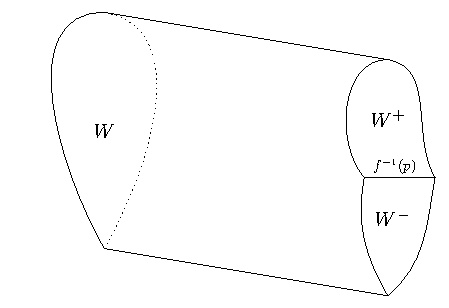
\includegraphics{figures/creasing2.pdf}
	\caption{Creasing homotopy}
	\label{F: creasing}
\end{figure}

If either $W \in PC^\Gamma_*(M)$ or $W \in PC_\Gamma^*(M)$, we have
\begin{equation}\label{E: bd crease}
	\bd(\Cre(W))\cong(D_x \sqcup -D_- \sqcup -D_+)\times_{(-1,1)} W \bigsqcup -D\times_{(-1,1)}\bd W = W \sqcup -W^- \sqcup -W^+ \sqcup -\Cre(\bd W),
\end{equation}
again interpreting these formulas in $PC^\Gamma_*(M)$ or $PC_\Gamma^*(M)$, respectively, by composing the pullback maps to $W$ with $r_W \colon W \to M$.
This first equality comes from our boundary formulas for $D$ and our Leibniz rules from \cref{S: orientations} and \cref{leibniz}.
For the second equality we use, for example, that $\pi$ is an orientation preserving diffeomorphism from $D_+ \cong [0,1)$ onto its image in $(-1,1)$, and so we have an orientation-preserving diffeomorphism $D_+\times_{(-1,1)} W \cong [0,1)\times_{(-1,1)} W = W^+$, and similarly in the co-oriented case.

\begin{comment}
	Next let us see how to use creasing in the context of chains and cochains.

	If $W \in PC_*^{\Gamma}(M)$ represented by $r_W \colon W \to M$, then $\Cre(W)$ is also compact and oriented, and we have a map $r_{\Cre(W)} = r_W\pi_W \colon W \to M$ with $\pi_W$ being the projection of $\Cre(W) = D\times_{(-1,1)}W$ to $W$.
	Thus $r_{\Cre(W)} \colon \Cre(W) \to M$ gives us a new element of $PC_*^\Gamma(M)$.
	If $W \in PC^*_\Gamma(M)$, then to get an element $\Cre(W) \in PC^*_\Gamma(M)$ we will need to assume that $\varphi \colon W \to (-1,1)$ is a composition of maps $W \xr{r_W}M \xr{\phi} (-1,1)$.
	We can then form the space $\Cre(W)$ as the pullback by $\phi r_W$ of $\pi: D \to (-1,1)$.
	As $\pi$ is proper and co-oriented, the pullback $\pi^* = \pi_W \colon \Cre(W) \to W$ will be proper and co-oriented by Lemma \ref{L: co-orientable pullback} and Definition \ref{D: pullback coorient}.
	We then let $r_{\Cre(W)} = r_W \pi^*$ to obtain an element of $\Cre(W) \in PC^*_\Gamma(M)$.
	By \cite[Propositions 7.4]{Joy12} and Theorem \ref{leibniz}, our boundary formulas for $\Cre(W)$ continue to hold as elements of $PC_*^{\Gamma}(M)$ or $PC^*_{\Gamma}(M)$.
\end{comment}

\begin{convention}\label{C: regular value setup}
	In order to crease an element of $PC_*^\Gamma(M)$ or $PC^*_\Gamma(M)$ represented by $r_W \colon W \to M$, we need a smooth map $\varphi \colon W \to (-1,1)$ so that the composite $\varphi: W \xr{r_W}M \xr{\phi} (-1,1)$ has $0$ as a regular value.
	In this case $M^0$ and $M^\pm$ are fiber products and thus manifolds with corners as in \cref{E: manifold decomposition}.
	Also as observed there, in this case $\varphi$ has $0$ as a regular value if and only if $r_W$ is transverse to $M^0$, in which case we also have $W^0 = M^0 \times_M W$ and $W^\pm = M^\pm \times_M W$.
	Unless noted, we will always assume this situation when working with creasing, i.e.\ that we have a fixed $\phi \colon M \to (-1,1)$ with $0$ a regular value and that creasing is defined with respect to the composition $\varphi = \phi r_W$ with $r_W$ transverse to $M^0$.
\end{convention}

To next promote the construction $\Cre(-)$ to an operator on $C_*^{\Gamma}(M)$ or $C^*_\Gamma(M)$, we will need \cref{L: pullback with Q} along with its following corollary.

\begin{comment}
	The lemma itself will also be important when we consider products below in Section \ref{S: products}.

	\begin{lemma}\label{L: pullback with Q}
		Let $M$ be a manifold without boundary.
		Suppose $T \in PC_*^\Gamma(M)$ (or $PC^*_\Gamma(M)$), and that $T \in Q(M)$.
		Then $T \times_M W \in Q(M)$ and $W \times_M T \in Q(M)$ for any $W$ in $PC_*^\Gamma(M)$ (or $PC^*_\Gamma(M)$) that is transverse to $T$.
	\end{lemma}
	\begin{proof}
		We consider only $T \times_M W$ as the arguments for $W \times_M T$ are the same.
		By assumption $T$ is the disjoint union of trivial and degenerate chains, so it suffices to consider independently the possibilities that $T$ is trivial or degenerate.

		If $\rho$ is a (co-)orientation reversing diffeomorphism of $T$ over $M$, then $\rho \times_M \id_W$ is a (co-)orientation reversing diffeomorphism of $T \times_M W$, by Joyce's construction in the oriented case and by Remark \ref{R: co-or restriction or switch} in the co-oriented case.

		Next assume that $T$ is degenerate, so in particular it has small rank.
		Recall that the tangent bundle of a fiber product is the fiber product of the tangent bundles \cite[Theorem 5.47]{Wed16}, and so the derivative is the fiber product of derivatives.
		Note that the fiber product of two linear maps, one with a non-trivial kernel must also have a non-trivial kernel: If $A,B$ are linear maps with a common codomain and $v \in \ker(A)$, then $(v,0)$ is in the kernel of the fiber product of $A$ and $B$.
		So if the differential of $r_W$ has non-trivial kernel everywhere so will the derivative of any fiber product with $r_W$.
		Thus $T \times_M W$ has small rank.

		Next we recall $\bd(T \times_M W) = (\bd T) \times_M W \bigsqcup \pm T \times_M (\bd W)$.
		We have just shown that $T \times_M (\bd W)$ must have small rank.
		As $T$ is degenerate, $\bd T$ is a disjoint of trivial and small rank manifolds over $M$, and so by the preceding arguments $(\bd T) \times_M W$ will be a union of trivial and small rank manifolds over $M$.
		Altogether, $T \times_M W$ is degenerate.
	\end{proof}
\end{comment}

\begin{corollary}\label{C: creasing Q}
	Let $M$ be a manifold without boundary.
	Suppose given $\phi \colon M \to (-1,1)$ with $0$ a regular value and $r_T \colon T \to M$ transverse to $M^0$.
	If $T \in Q(M)$ then so are $T^+$, $T^-$, $T^0$, and $\Cre(T)$.
\end{corollary}

\begin{proof}
	As observed in \cref{C: regular value setup}, with our assumptions about $\varphi$ the spaces $T^\pm$ and $T^0$ are fiber products over $M$ of $T$ with $M^\pm$ and $M^0$.
	So in this case the claim follows from the \cref{L: pullback with Q}.

	For $\Cre(T)$, the pullback projection $\pi \colon \Cre(T) \to T$ is of small rank, as $\dim(\Cre(T))>\dim(T)$, from which it follows that $r_{\Cre(T)} = r_T\pi$ is of small rank.
	We also have $\bd \Cre(T) = T \sqcup - T^+ \sqcup -T^- \sqcup -\Cre(\bd T)$.
	By assumption and the preceding paragraph, $T, T^\pm \in Q(M)$ and by the preceding sentence $\Cre(\bd T)$ is of small rank.
	Thus all components of $\bd \Cre(T)$ are trivial or of small rank, and so $\Cre(T)$ is degenerate.
\end{proof}

\begin{proposition}
	Let $M$ be a manifold without boundary.
	Suppose given $\phi \colon M \to (-1,1)$ with $0$ a regular value.
	If $V$ and $W$ are any two representatives of $\uW \in C_*^\Gamma(M)$ whose reference maps are transverse to $M^0$, then $\Cre(V)$ and $\Cre(W)$ represent the same element of $C_*^\Gamma(M)$.
	Thus if the equivalence class $\uW$ contains any representative that is transverse to $M^0$, there is a well-defined element $\underline{\Cre(W)} \in C_*^\Gamma(M)$.
	Similarly for $C^*_\Gamma(M)$.
\end{proposition}

\begin{proof}
	The proofs for chains and cochains are the same, so we provide that with chains.

	If $r_V \colon V \to M$ and $r_W \colon W \to M$ represent the same class in $C_*^\Gamma(M)$ then $V \sqcup -W \in Q_*(M)$, and if $V$ and $W$ are both transverse to $M^0$ then so is $V \sqcup -W$.
	So $\Cre(V\sqcup-W)$ is defined, and by \cref{C: creasing Q}, $\Cre(V \sqcup -W) \in Q_*(M)$.
	Using our convention that all creasing maps are compositions of the fixed $\phi \colon M \to (-1,1)$ with the reference maps and the properties of fiber product orientations, we have $\Cre(V \sqcup -W) = \Cre(V) \sqcup \Cre(-W) = \Cre(V) \sqcup -\Cre(W)$.
	Thus $\Cre(V)$ and $\Cre(W)$ represent the same element of $C_*^\Gamma(M)$.
\end{proof}

Finally, we come to the punchline of creasing:

\begin{theorem}\label{T: cohomology creasing}
	Let $M$ be a manifold without boundary.
	Suppose $\uW \in H_*^\Gamma(M)$ and that $\uW$ has a representative $r_W \colon W \to M$ that is transverse to $M^0$, defined with respect to some $\phi \colon M \to (-1,1)$ with $0$ a regular value.
	Then $\uW = \underline{W^+} + \underline{W^-} \in H_*^\Gamma(M)$.
	Similarly for $H^*_\Gamma(M)$.
\end{theorem}

\begin{proof}
	Again the proofs for homology and cohomology are the same so we focus on homology.

	We have seen that, with our assumptions, $\uW$ yields a well-defined element $\underline{\Cre(W)}$ represented by $\Cre(W)$.
	Computing in $C_*^\Gamma(M)$ we have
	\begin{align*}
		\bd \underline{\Cre(W)}& = \underline{\bd \Cre(W) }\\
		& = \underline{W \sqcup -W^+ \sqcup -W^- \sqcup -\Cre(\bd W)}\\
		& = \uW -\underline{W^+}-\underline{W^-}.
	\end{align*}
	In the last line we have used that $\underline{\bd W} = 0$ so that $\bd W \in Q_*(M)$ and hence $\Cre(\bd W) \in Q_*(M)$ by \cref{C: creasing Q} and $\underline{\Cre(\bd W)} = 0 \in C_*^\Gamma(M)$.
	The theorem follows.
\end{proof}

\begin{comment}
	Let $f \colon W \to \R$ and $p$ be a regular value of $f$.
	Define $W^+$ to be $f^{-1} [p, \infty)$ and $W^-$ to be $f^{-1} (-\infty, p]$.
	By Theorem~1 of \cite{Lipy14} (and
	also transversality as developed in in Section 6 of \cite{Joy12}), $W^+$ and $W^-$ are manifolds with corners.
	The following is Lemma~9 of \cite{Lipy14}.

	\begin{proposition}\label{P: creasing}
		Let $f \colon W \to \R$ and $p$ be a regular value of $f$.
		There is a manifold-with corners structure on the topological manifold $W \times [0,1]$, called the creasing of $W$ at $p$,
		whose boundary is the disjoint union of $W$ with its orientation
		reversed, $W^+$, $W^-$ and the creasing of ${\bd W}$ at $p$.
	\end{proposition}

	We denote the creasing of $W$ at $p$ by $\Cre(W)$, suppressing $f$ and $p$ from notation.
	See Figure~\ref{F: creasing} for a sketch of a creasing of the teardrop manifold.
\end{comment}